\section{\benchmark Dataset}
\label{sec:dataset}


\begin{figure}[t]
\captionsetup{skip=1mm}
\centering
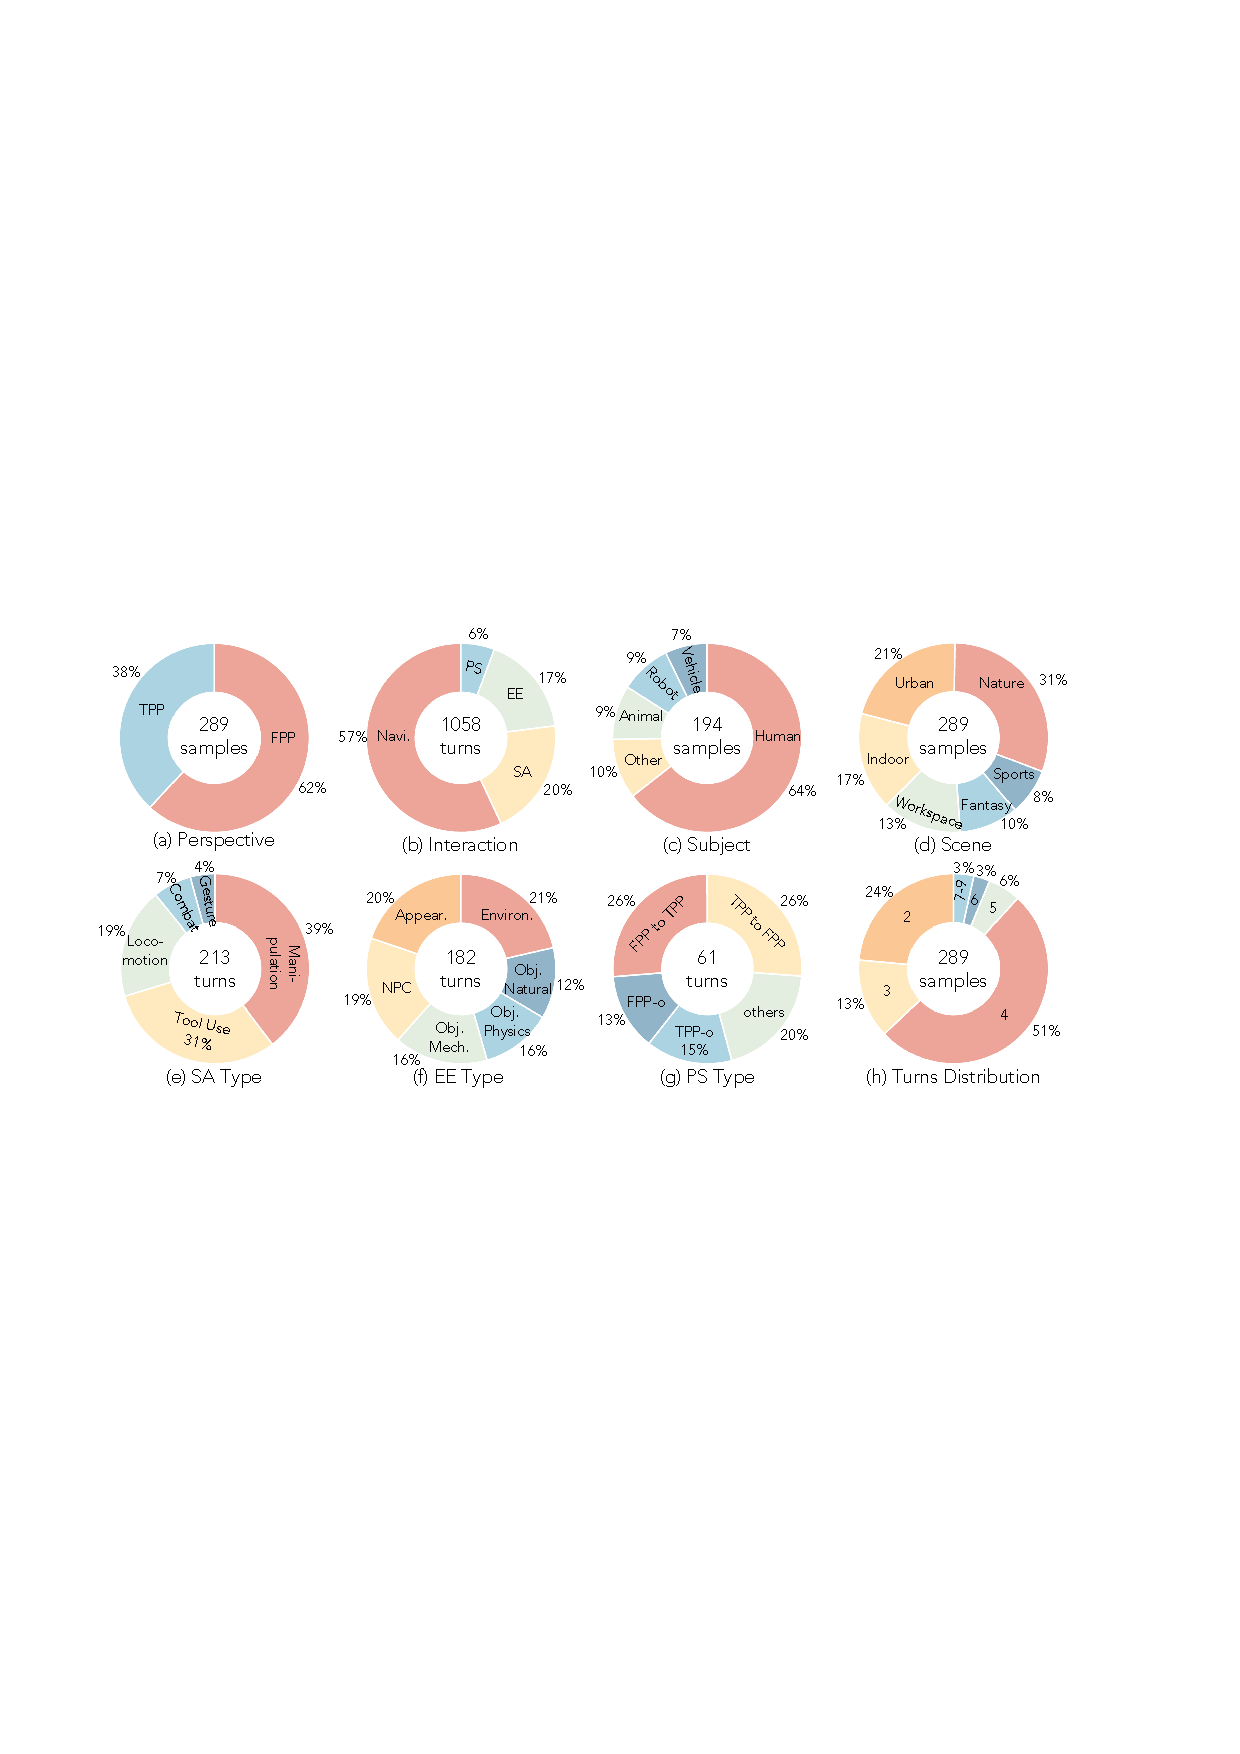
\includegraphics[width=0.95\linewidth]  {figures/category_pie_new.pdf}%
\caption[Dataset composition across eight axes]{Dataset composition of \benchmark across eight axes. We discuss these in \cref{sec:statistics}.}
\vspace{-2mm}
\label{fig:dataset_distribution}
\end{figure}


An interactive world model~\cite{ha2018world,lecun2022path} acts as a conditional generator that predicts the next observation $o_{t+1}$ given the historical observation $o_{\le t} = (o_0, \dots, o_t)$ and the action $a_{\le t} = (a_0, \dots, a_t)$:
\begin{equation}
    o_{t+1} \sim f_\theta(o_{t+1}|o_{\le t}, a_{\le t}).
\label{eq:world_model}
\end{equation}
To systematically evaluate this process, every case in \benchmark decomposes the inputs into two components: a \textbf{World Setting} $\mathcal{W}$ that defines the initial world state $o_0$, and an \textbf{Interaction sequence} $\mathcal{I} = (a_0, a_1, \dots, a_{T-1})$ that specifies the user control signals spanning $T$ consecutive turns.

\subsection{Dataset Construction}
\label{sec:ontology}

\myparagraph{World Settings.}
A world setting $\mathcal{W}$ is defined by four attributes:
\textbf{1)~Scene}, the environment type, spatial layout, and inherent dynamics, including both elements visible in the initial frame (\eg, terrain, buildings) and offscreen elements expected to appear during interaction (\eg, a river behind the camera);
\textbf{2)~Style}, the rendering appearance, such as realistic, cartoon, anime, cinematic, CG, or oil painting;
\textbf{3)~Perspective}, either first- or third-person;
and \textbf{4)~Subject}, the primary entity in the scene, such as a human, animal, vehicle, or robot. The subject attribute applies to all third-person cases and first-person cases where the viewer holds or controls a visible entity (\eg, a tool or an ego robot arm); environment-only first-person scenes have no associated subject.
These four attributes are composed into an \textbf{environment prompt} (Scene + Style) and a \textbf{subject prompt} (Perspective + Subject), which together with an initial frame form the input to each evaluated model.
Initial frames are generated by Nano Banana~2~\cite{google2025nanobanana2} and GPT-Image-1.5~\cite{openai2025gptimage}, supplemented by web-collected and manually captured images. All initial frames undergo manual verification for quality control.


\myparagraph{Interactions.}
Each case specifies a multi-turn interaction sequence drawn from four complementary types that can be freely composed within a single case, as shown in \cref{fig:teaser} (top).
\textbf{1)~Navigation} governs camera or ego-agent motion through four \emph{translational} controls \texttt{W}/\texttt{S}/\texttt{A}/\texttt{D} and four \emph{rotational} controls $\leftarrow$/$\rightarrow$/$\uparrow$/$\downarrow$, composable into compound actions such as \texttt{W}+$\leftarrow$. The same key drives the camera in first-person mode and the subject in third-person mode. Trajectories span six path topologies for motion diversity (\cref{app:nav_coverage}).
\textbf{2)~Subject Action} covers actions performed by the primary subject, including manipulation, locomotion, tool use, combat, and gestural interaction.
\textbf{3)~Event Editing} covers externally imposed changes to the environment, such as weather transitions, time-of-day shifts, object appearances, \etc
\textbf{4)~Perspective Switching} covers transitions between first- and third-person views, including same-subject switches, multi-subject switches, and scope mode transitions.

\myparagraph{Case Construction.}
Construction follows a setting-first principle: annotators design a world setting and then derive interaction sequences that are physically executable and semantically coherent within it (\eg, manipulation in a kitchen, weather transitions outdoors, and reasonable navigation trajectories). Multi-turn sequences respect causal ordering. We apply stratified sampling across scene, style, perspective, subject, and interaction type to ensure diverse coverage, with all selected cases undergoing manual review for prompt-frame consistency and inter-turn coherence.

\subsection{Dataset Statistics}
\label{sec:statistics}


\benchmark comprises \numvideo cases spanning \numturn interaction turns, with first-person cases at $62\%$ and third-person at $38\%$, see \cref{fig:dataset_distribution}~\!(a). Navigation is the most prevalent interaction ($57\%$), followed by subject action ($20\%$), event editing ($17\%$), and perspective switching ($6\%$), as shown in \cref{fig:dataset_distribution}~\!(b).

\myparagraph{Scene, Subject, and Style Diversity.} Scenes span six categories, led by nature ($31\%$) and urban environments ($21\%$), with indoor ($17\%$), works ($13\%$), fantasy ($10\%$), and sports ($8\%$) settings completing the spectrum, see \cref{fig:dataset_distribution}~\!(d). Across the $194$ cases with an explicit subject, humans dominate ($64\%$), followed by animals ($9\%$), robots ($9\%$), vehicles ($7\%$), and $10\%$ miscellaneous objects (\cref{fig:dataset_distribution}~~(c)). Photorealistic rendering covers $52\%$ of the cases, while the remaining $48\%$ span styles including anime, cartoon, CG, oil painting, ink wash, pencil sketch, and flat or abstract styles.

\myparagraph{Interaction Sub-type Taxonomy.}
As shown in \cref{fig:dataset_distribution}~~(e)(g), subject action is categorized into five sub-types, dominated by manipulation ($39\%$) and tool use ($31\%$), with locomotion, combat, and gestures comprising the remainder. Event editing covers six relatively balanced sub-types, including environment changes ($21\%$), appearance-state changes ($20\%$), NPC motion ($19\%$), and three types of object-state transitions involving mechanical, physical, and natural phenomena. Perspective switching consists of $61$ turns, including cross-perspective switches with each direction at $26\%$, intra-perspective switches(denoted by ``-o'' in the figure) accounting for $28\%$ in total, and other switches such as TPP-to-scope.

\myparagraph{Multi-turn Interaction Depth.}
Each case spans 2-9 interaction turns with an average of $3.7$, as shown in \cref{fig:dataset_distribution}~~(h). Four-turn cases are the most common ($51\%$) and mostly correspond to navigation trajectories, whereas the $12\%$ of longer 5--9-turn cases typically interleave subject action with event editing. Such multi-turn structure probes temporal consistency and long-horizon coherence, which single-turn benchmarks cannot assess. Further breakdowns of navigation coverage, evaluation activation, and lexical diversity are provided in \cref{app:dataset}.
